\documentclass[a4paper,12pt]{article}
\usepackage[utf8]{vietnam}
\usepackage{hyperref}
\usepackage{graphicx}
\usepackage{xcolor}
\usepackage{subfigure}
\usepackage{float}
\usepackage{caption}
\usepackage{placeins}
\makeatletter
\setlength{\@fptop}{0pt}
\makeatother
\hypersetup{
	pdfborder = {0 0 0}
}
\title{\textbf{Báo cáo Project cuối kì \\ IT3290 - Thực hành cơ sở dữ liệu}}
\author{}
\date{}
\begin{document}
\maketitle
\noindent
\textbf{Học phần} Thực hành cơ sở dữ liệu - IT290 \textbf{- Mã lớp} 130993\\
\textbf{Nhóm HUSTFood:}
\begin{enumerate}
	\item Phan Minh Anh Tuấn (20205227)
	\item Nguyễn Thị Hoài Linh (20205231)
	\item Vũ Minh Long (20200373)
	\item Đàm Ngọc Khánh (20205207)
\end{enumerate}\large
\newpage
\tableofcontents
\newpage
\section{Tổng quan Database}
\begin{figure}[ht!]
	\centerline{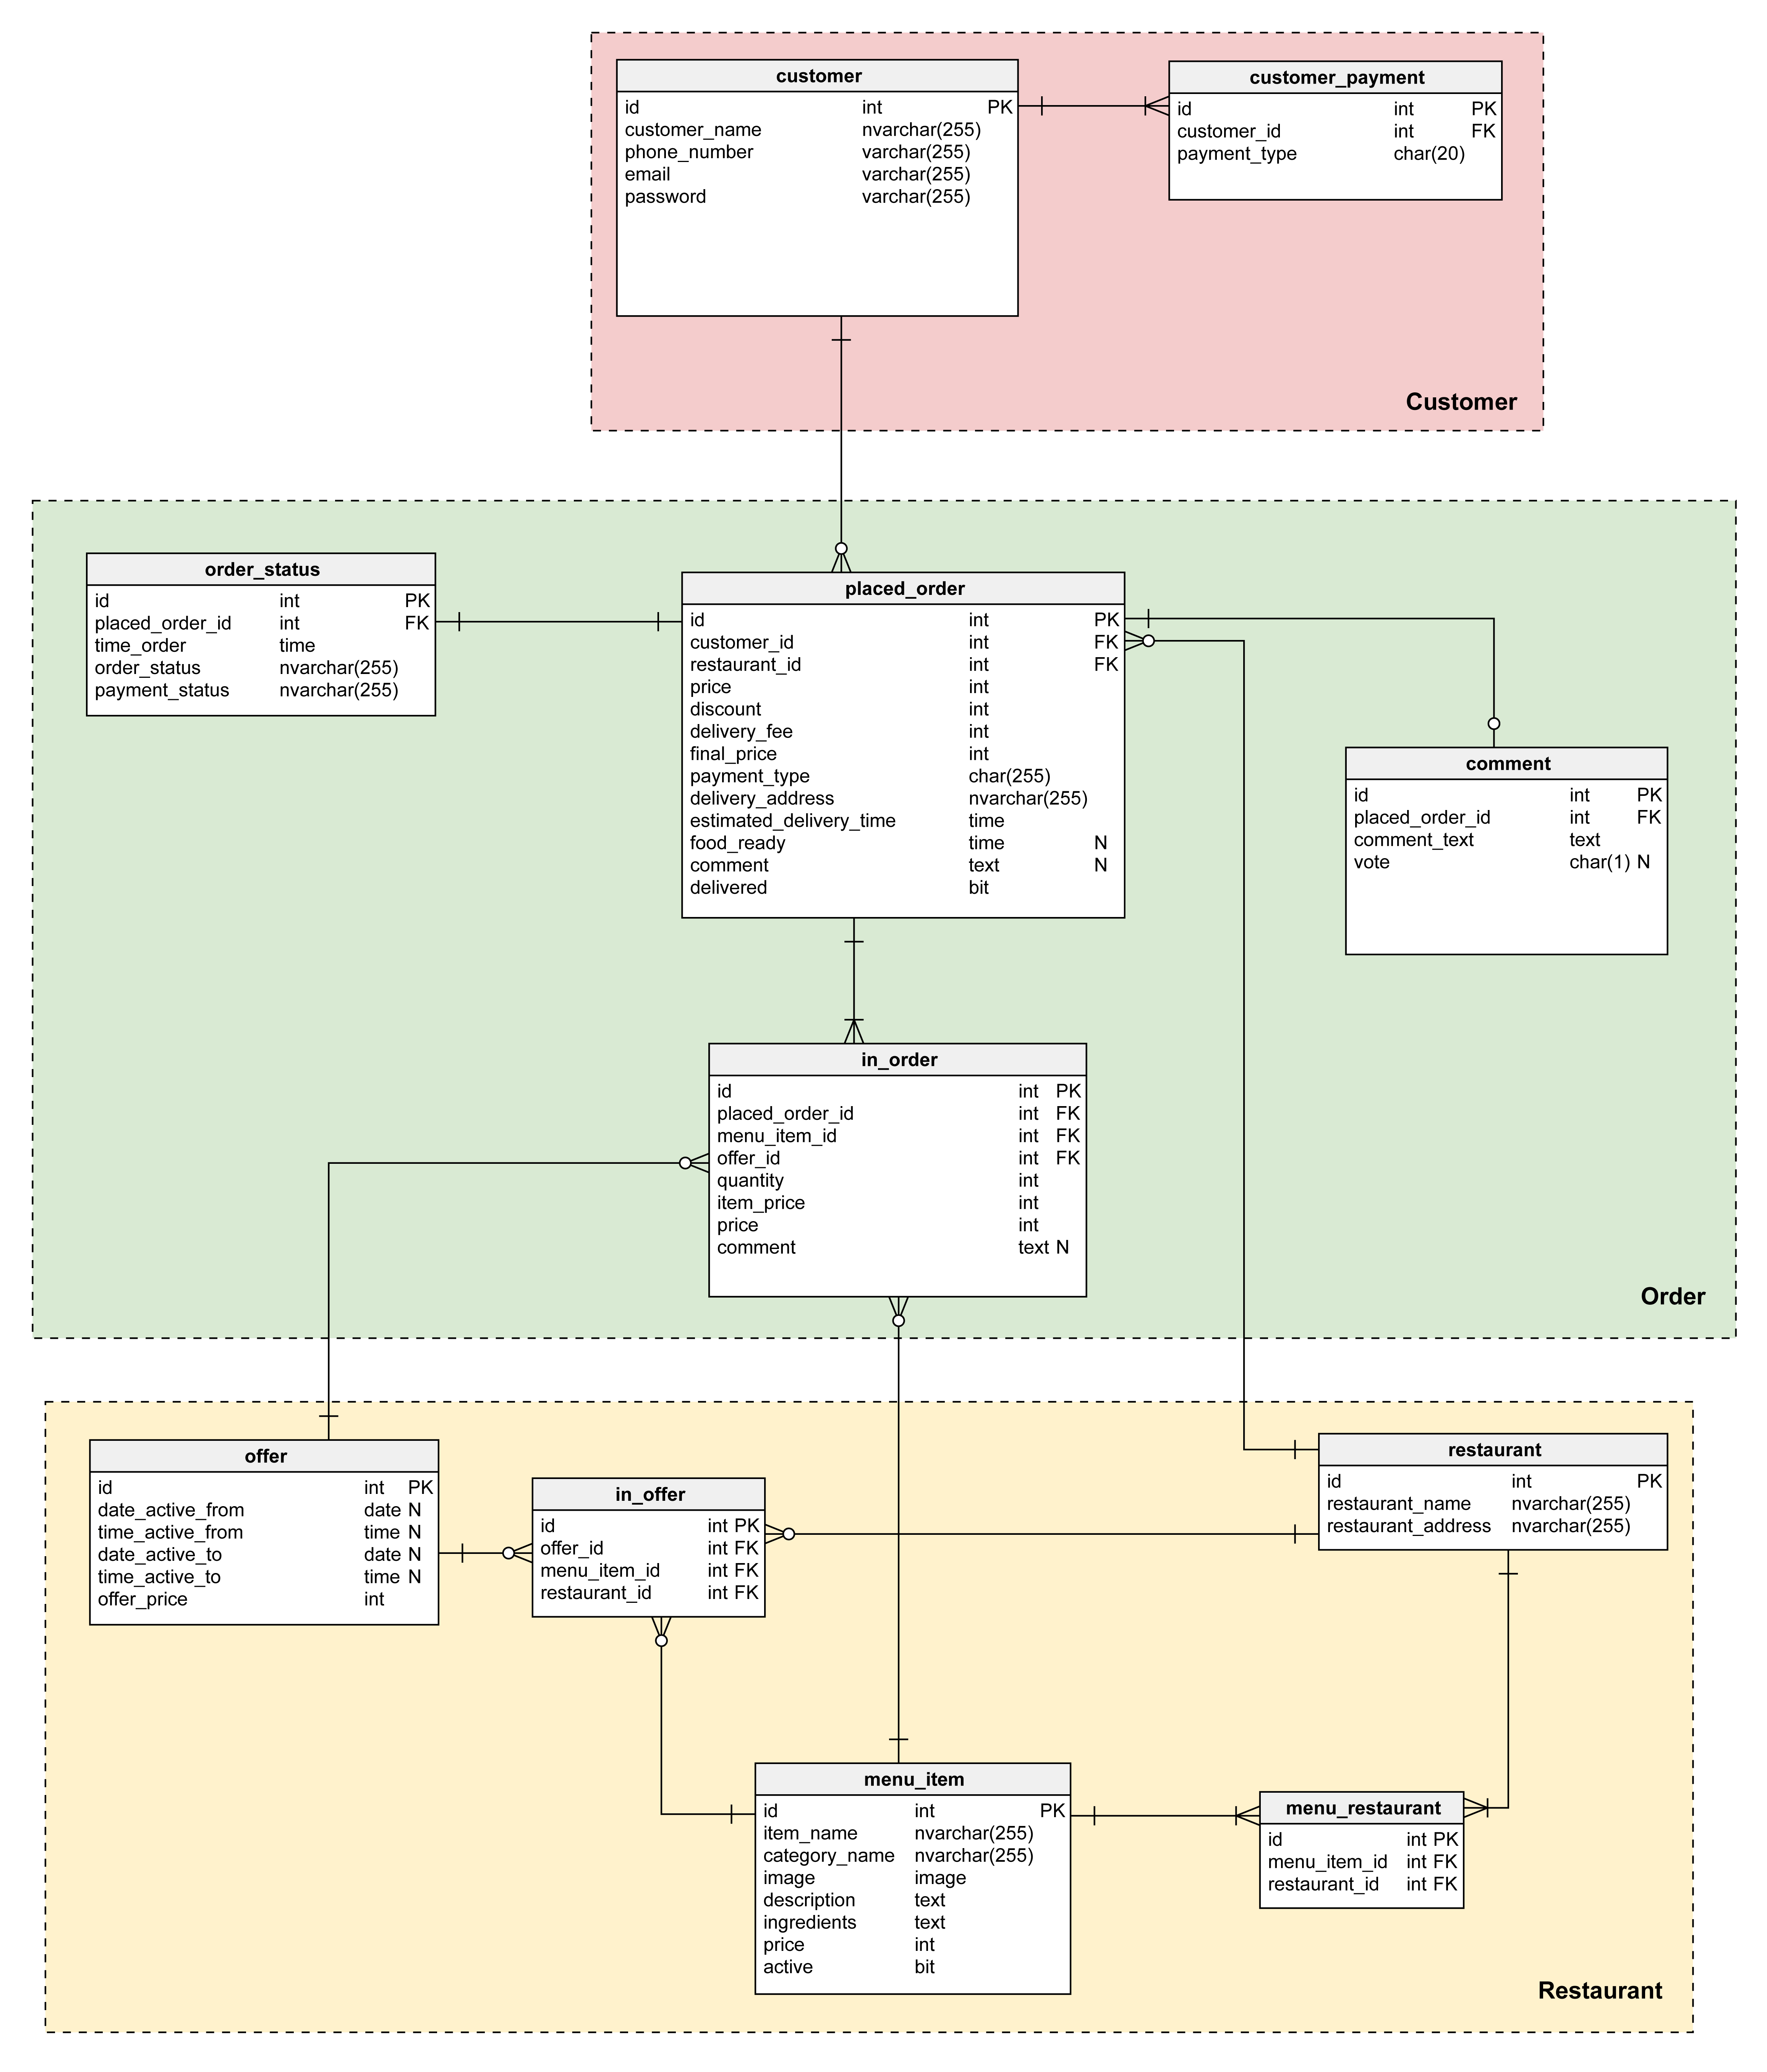
\includegraphics[width=0.9\textwidth]{sql.png}}
	\label{fig:ass1}
	\caption{Database HUSTFood}
\end{figure}
\clearpage
\section{Customer}
\begin{figure}[ht!]
	\centerline{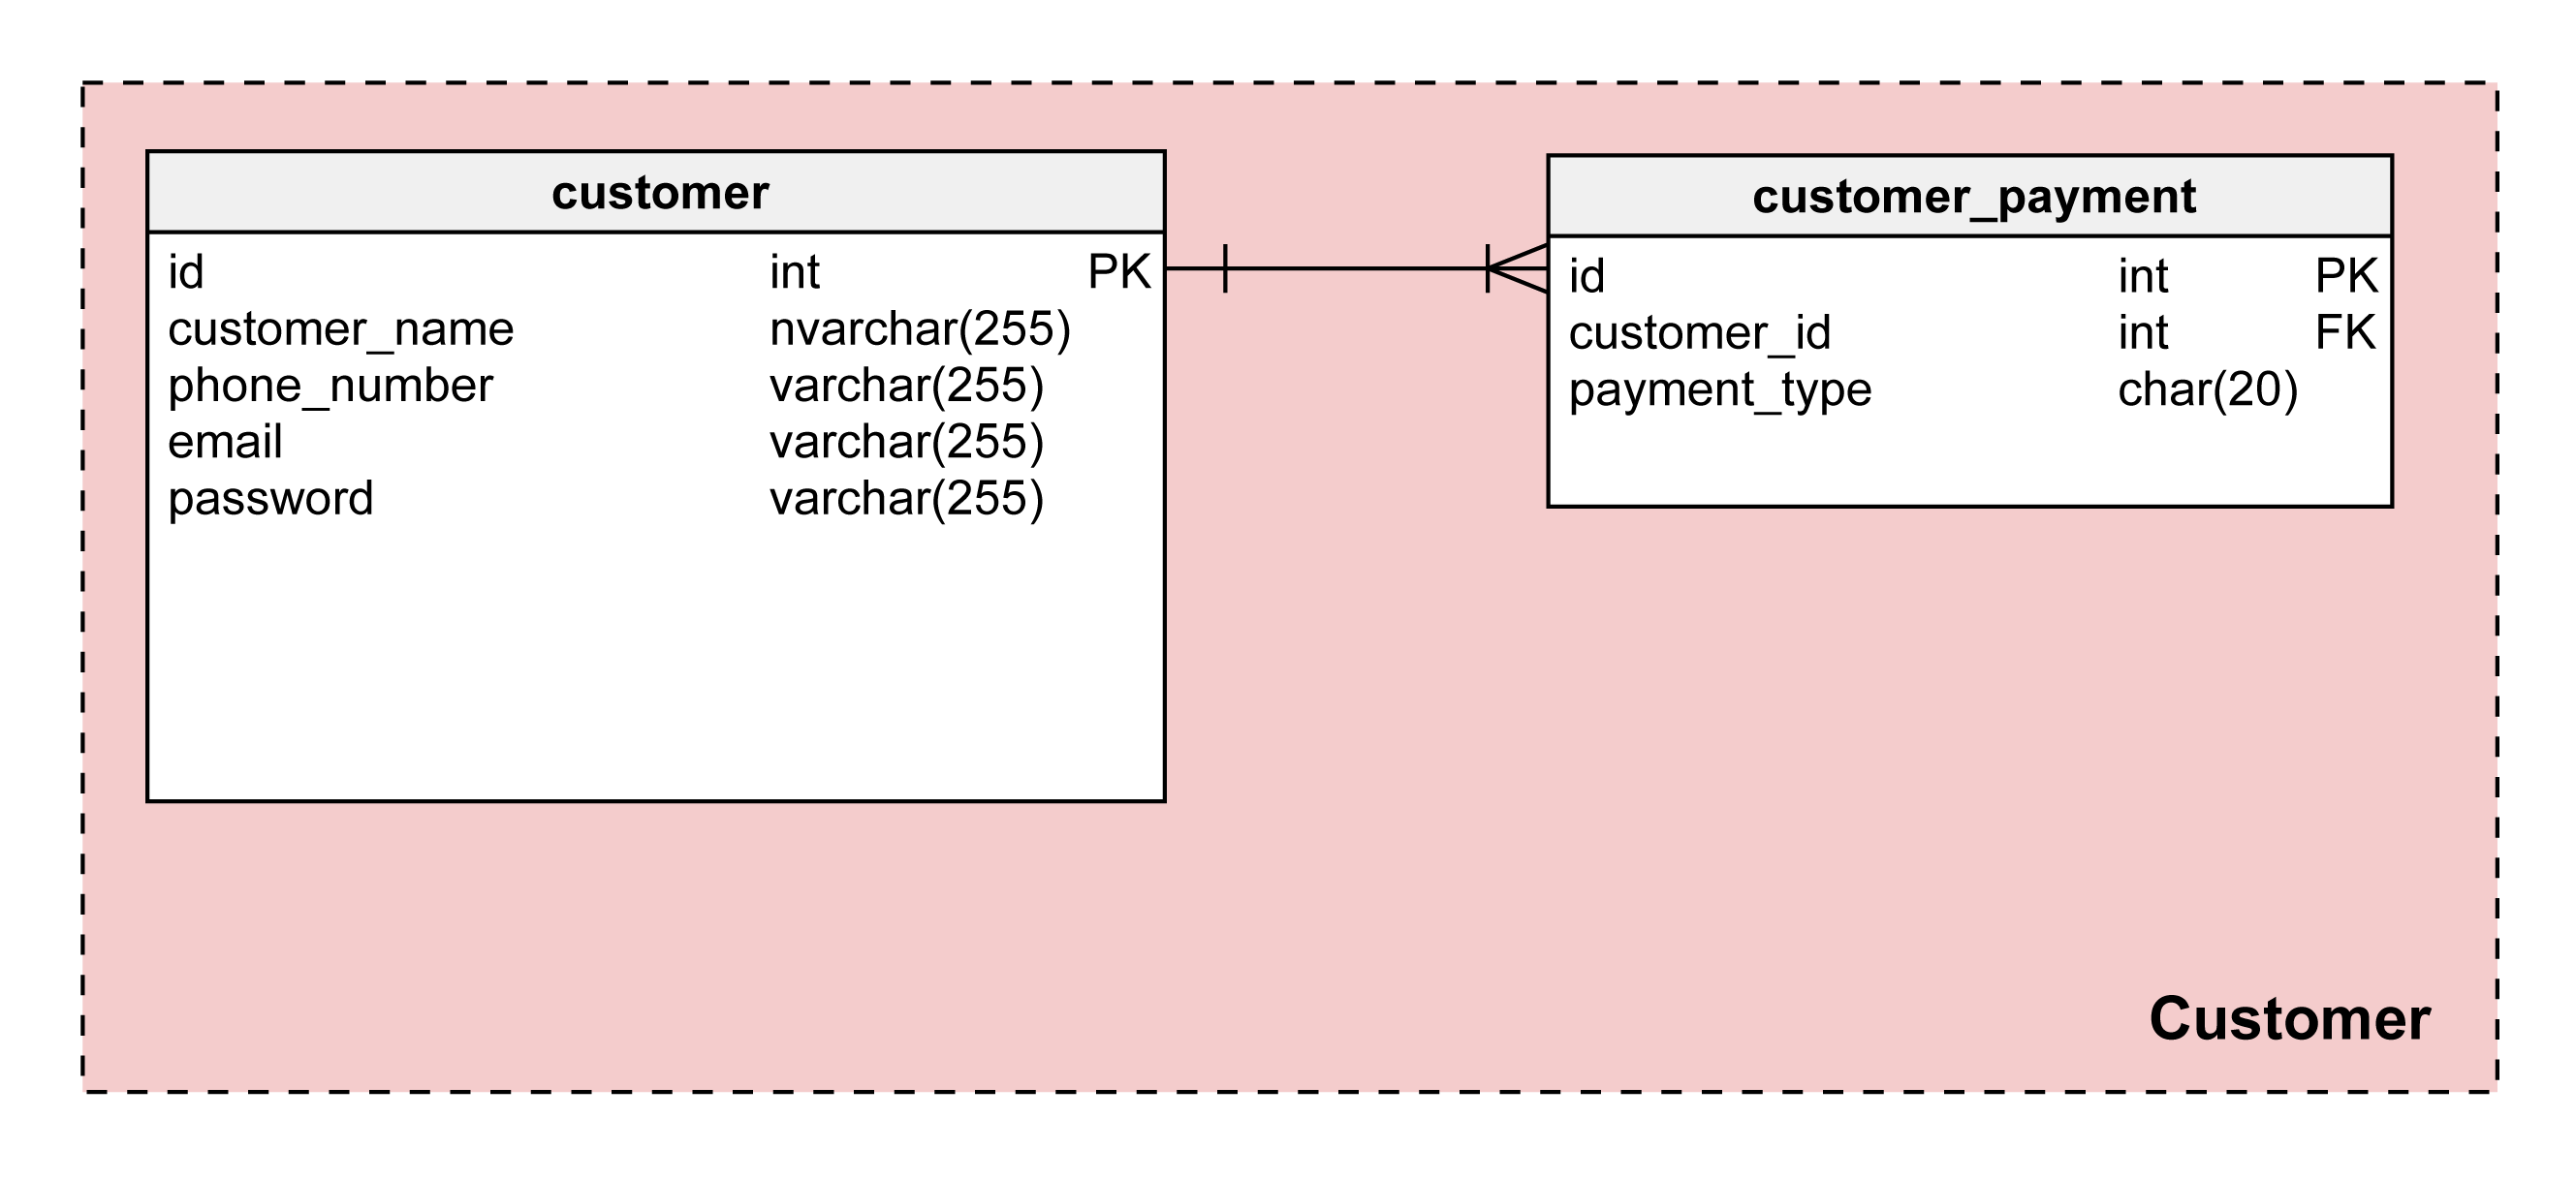
\includegraphics[width=1\textwidth]{customer.png}}
	\label{fig:ass1}
	\caption{Các bảng trong Customer}
\end{figure}
\noindent
\subsection{Customer}
\begin{itemize}
	\item \textbf{id:} Mã khách hàng (Primary key)
	\item \textbf{customer$\_$name:} Tên khách hàng
	\item \textbf{phone$\_$number:} Số điện thoại khách hàng
	\item \textbf{email:} Mail khách hàng
	\item \textbf{password:} Mật khẩu tài khoản
\end{itemize}
\subsection{Customer\_payment}
\begin{itemize}
	\item \textbf{id:} (Primary key)
	\item \textbf{customer\_id:} Foreign key customer(id)
	\item \textbf{payment\_type:} Phương thức thanh toán
\end{itemize}
\clearpage
\section{Order}
\begin{figure}[ht!]
	\centerline{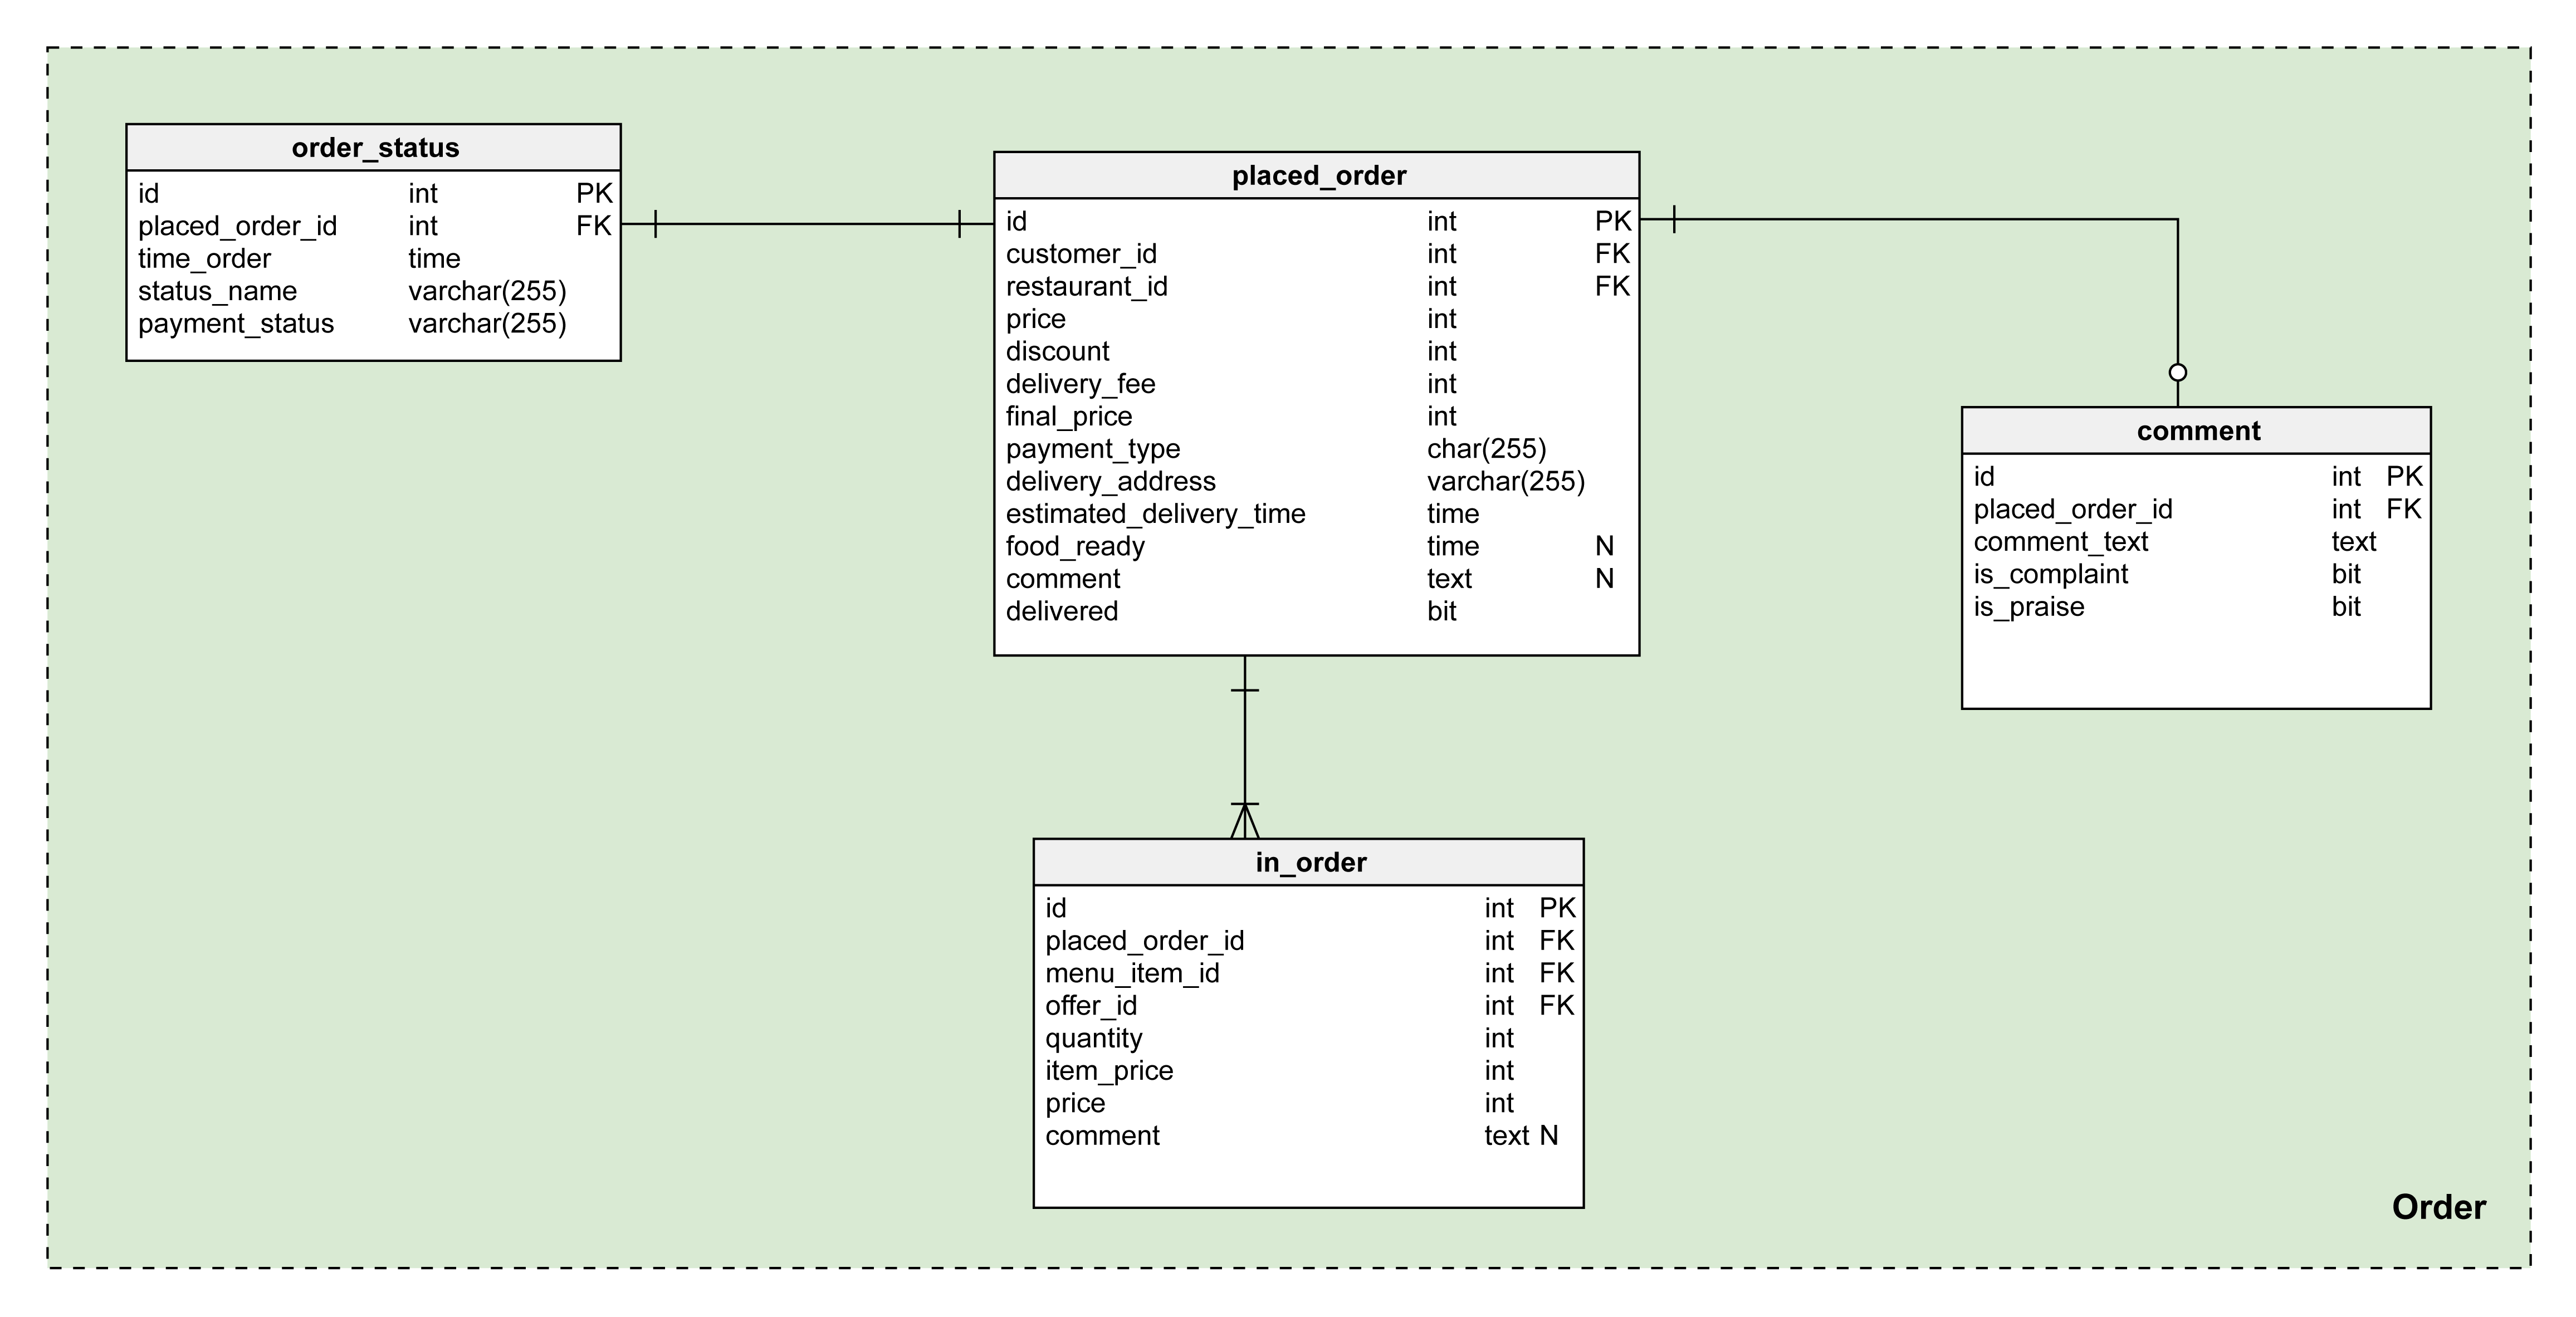
\includegraphics[width=1\textwidth]{order.png}}
	\label{fig:ass1}
	\caption{Các bảng trong Order}
\end{figure}
\subsection{Placed Order}
\begin{itemize}
	\item \textbf{id:}
	\item \textbf{customer\_id:} Foreign key customer(id)
	\item \textbf{restaurant\_id:} Foreign key restaurant(id)
	\item \textbf{price:} Giá ban đầu
	\item \textbf{discount:} Giảm giá 
	\item \textbf{delivery\_fee: }Phí vận chuyển
	\item \textbf{final\_price:} Giá phải trả
	\item \textbf{payment\_type:} Hình thức thanh toán
	\item \textbf{delivery\_address:} Địa chỉ giao hàng 
	\item \textbf{estimated\_delivery\_time:} Thời gian dự kiến giao hàng
	\item \textbf{food\_ready:} Đồ ăn đã sẵn sàng chưa
	\item \textbf{comment:} Lưu ý của khách hàng
	\item \textbf{deliveried:} Đã được giao hay chưa
\end{itemize}
\subsection{Order status}
\begin{itemize}
	\item \textbf{id:} Mã trạng thái đơn hàng
	\item \textbf{placed\_order\_id:} Mã đơn đặt hàng (Foreign key placed\_order(id))
	\item \textbf{time\_order:} Thời gian đặt hàng
	\item \textbf{status\_name:} Trạng thái đơn hàng (Thêm vào giỏ/ Xác nhận/ Đã thanh toán / Đã giao)
	\item \textbf{payment\_status:} Trạng thái thanh toán
\end{itemize}
\subsection{In order}
\begin{itemize}
	\item \textbf{id:} Mã
	\item \textbf{placed\_order\_id:} Mã đơn đặt hàng (Foreign key placed\_order(id))
	\item \textbf{offer\_id:} Mã ưu đãi (Foreign key offer(id))
	\item \textbf{menu\_item\_id:} Mã mặt hàng (Foreign key menu\_item(id))
	\item \textbf{quantity:} Số lượng mua
	\item \textbf{item\_price:} Giá lẻ
	\item \textbf{price:} Tổng giá
	\item \textbf{Comment:} Lưu ý của khách hàng (giao 11h30 chả hạn)
\end{itemize}
\subsection{Comment}
\begin{itemize}
	\item \textbf{id:}
	\item \textbf{placed\_order\_id:} Mã đơn đặt hàng (Foreign key placed\_order(id))
	\item \textbf{customer\_id:} Mã khách hàng (Foreign key customer(id))
	\item \textbf{comment\_text:} Đánh giá của khách hàng
	\item \textbf{is\_complaint:} Có phải lời phàn nàn không?
	\item \textbf{is\_complaint:} Có phải lời khen không?
\end{itemize}
\clearpage
\section{Restaurant}
\begin{figure}[ht!]
	\centerline{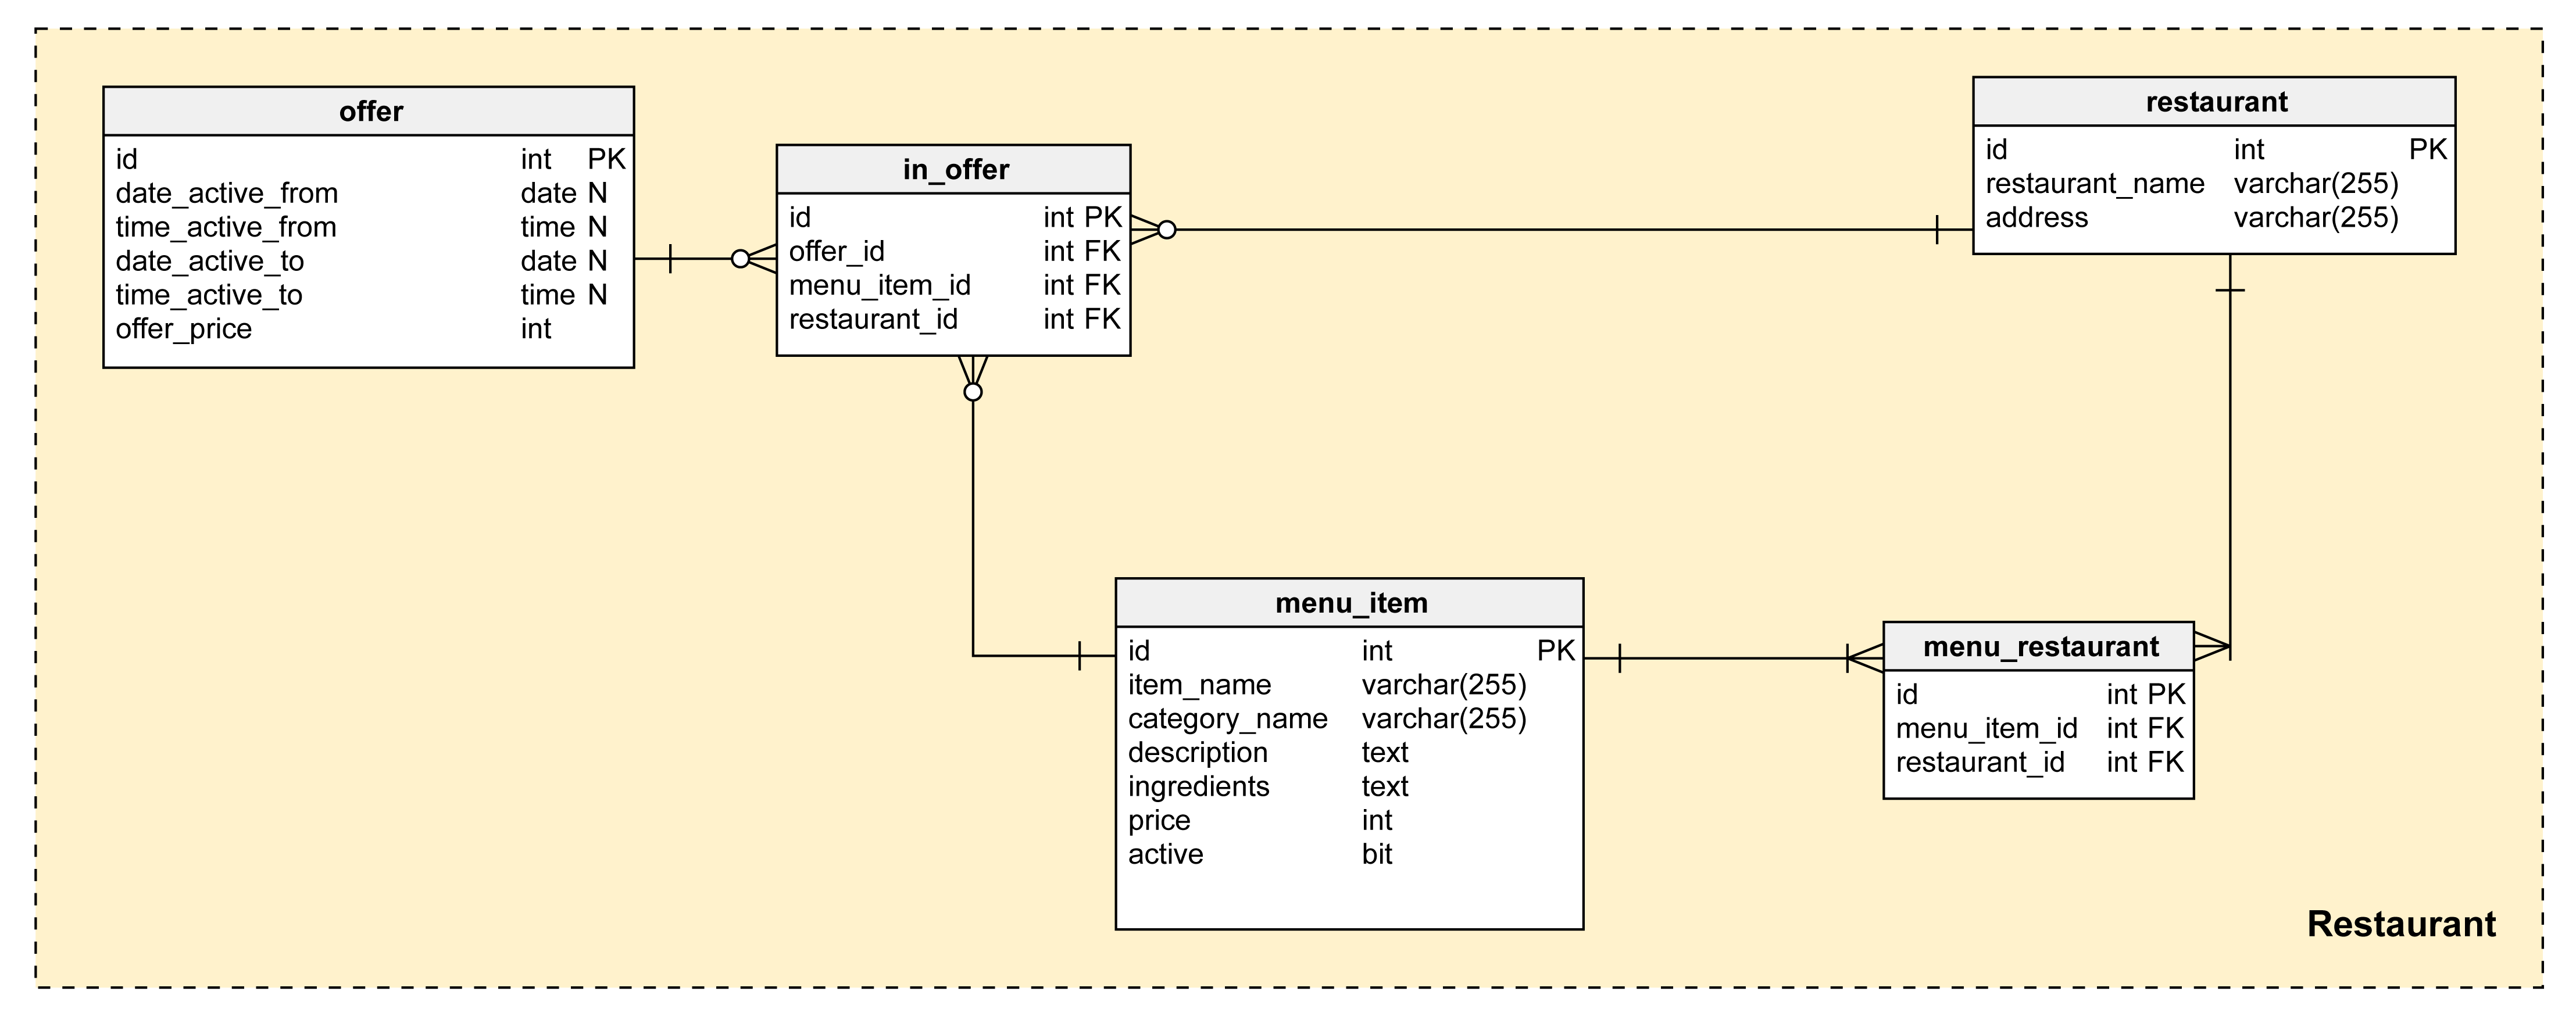
\includegraphics[width=1\textwidth]{restaurant.png}}
	\label{fig:ass1}
	\caption{Các bảng trong Restaurant}
\end{figure}
\subsection{Menu item}
\begin{itemize}
	\item \textbf{id:} Mã món ăn (Primary key)
	\item \textbf{item\_name:} Tên món ăn
	\item \textbf{category\_name:} Phân loại
	\item \textbf{description:} Mô tả
	\item \textbf{ingredients:} Nguyên liệu
	\item \textbf{price:} Giá
	\item \textbf{active:} Tình trạng mặt hàng (còn hay hết)
\end{itemize}
\subsection{Restaurant}
\begin{itemize}
	\item \textbf{id: } Mã nhà hàng
	\item \textbf{restaurant\_name:} Tên nhà hàng
	\item \textbf{address:} Địa chỉ
\end{itemize}
\subsection{Menu restaurant}
\begin{itemize}
	\item \textbf{id: } Mã nhà hàng
	\item \textbf{restaurant\_name:} Tên nhà hàng
	\item \textbf{address:} Địa chỉ
\end{itemize}
\subsection{Offer}
\begin{itemize}
	\item \textbf{id: } Mã ưu đãi
	\item \textbf{data\_active\_from:} Ngày bắt đầu kích hoạt
	\item \textbf{time\_active\_from:} Giờ bắt đầu kích hoạt
	\item \textbf{data\_active\_to:} Ngày kết thúc kích hoạt
	\item \textbf{time\_active\_to:} Giờ kết thúc kích hoạt
	\item \textbf{offer\_price:} Giá trị ưu đãi
\end{itemize}
\subsection{In offer}
\begin{itemize}
	\item \textbf{id: } Mã
	\item \textbf{offer\_id: } Foreign key offer(id)
	\item \textbf{menu\_item\_id: } Foreign key menu\_item(id)
	\item \textbf{restaurant\_id: } Foreign key restaurant(id)
\end{itemize}
\end{document}